\documentclass[11pt]{article} % use larger type; default would be 10pt

\usepackage[utf8]{inputenc} % set input encoding (not needed with XeLaTeX)

%%% Examples of Article customizations
% These packages are optional, depending whether you want the features they provide.
% See the LaTeX Companion or other references for full information.

%%% PAGE DIMENSIONS
\usepackage{geometry} % to change the page dimensions
\geometry{a4paper} % or letterpaper (US) or a5paper or....
% \geometry{margin=2in} % for example, change the margins to 2 inches all round
% \geometry{landscape} % set up the page for landscape
%   read geometry.pdf for detailed page layout information

\usepackage{graphicx} % support the \includegraphics command and options
%%% PACKAGES
\usepackage{booktabs} % for much better looking tables
\usepackage{array} % for better arrays (eg matrices) in maths
\usepackage{paralist} % very flexible & customisable lists (eg. enumerate/itemize, etc.)
\usepackage{verbatim} % adds environment for commenting out blocks of text & for better verbatim
\usepackage{subfig} % make it possible to include more than one captioned figure/table in a single float
% These packages are all incorporated in the memoir class to one degree or another...

\usepackage{fancyhdr} % This should be set AFTER setting up the page geometry
\pagestyle{fancy} % options: empty , plain , fancy
\renewcommand{\headrulewidth}{0pt} % customise the layout...
\lhead{}\chead{}\rhead{}
\lfoot{}\cfoot{\thepage}\rfoot{}

%%% SECTION TITLE APPEARANCE
\usepackage{sectsty}
\allsectionsfont{\sffamily\mdseries\upshape} % (See the fntguide.pdf for font help)
% (This matches ConTeXt defaults)

%%% ToC (table of contents) APPEARANCE
\usepackage[nottoc,notlof,notlot]{tocbibind} % Put the bibliography in the ToC
\usepackage[titles,subfigure]{tocloft} % Alter the style of the Table of Contents
\usepackage{framed}
\renewcommand{\cftsecfont}{\rmfamily\mdseries\upshape}
\renewcommand{\cftsecpagefont}{\rmfamily\mdseries\upshape} % No bold!

%%% END Article customizations

%%% The "real" document content comes below...

\title{Basics of Probability}
\author{Dublin \texttt{R}}


\begin{document}
\maketitle
%-----------------------------------------------------------------------------------------------------------------------------------%
\tableofcontents
\section{Overview}

\begin{itemize}
\item Overview
\item Basics of Probability (some definitions, the \texttt{prob} package) 
\item Dice Rolls and the Birthday Distribution ( histograms )
\item Gambler's Ruin ( plotting functions )
\item The Monty Hall Problem 
 
\item Probability Distributions (continuous and discrete distributions)
\end{itemize}
Book: \textbf{\textit{Introduction to Probability and Statistics using R}} by G Kerns \\ (downloadable for free online) We will use chapters 4,5 and 6. \\ \bigskip
Packages: The \texttt{prob} package (for the first part only).

\begin{framed}
\begin{verbatim}
install.packages("prob")
library(prob)
\end{verbatim}
\end{framed}
\newpage
\section{Some Probability Definitions}

\begin{description}
\item[Random Experiment] A random experiment is one whose outcome is determined by chance, with an outcome that may not be predicted with certainty beforehand. Common examples are coin tosses and dice rolls.
\item[Sample Space] For a random experiment E, the set of all possible outcomes of E is called the sample space and
is denoted by the letter S . For a coin-toss experiment, S would be the results ``Head” and ``Tail”, for a  single roll of a die it is the numbers 1 to 6.
\item[Events] An event $A$
 is merely a collection of outcomes, or in other words, a subset of the sample space.
\end{description}

\newpage
\section{The Birthday Paradox}
\subsection{The Birthday function}
The \texttt{R} command \texttt{pbirthday()} computes the probability of a coincidence of a number of randomly chosen people sharing a birthday, given that there are $n$ people to choose from.
Suppose there are four people in a room. The probability of two of them sharing a birthday can be computed as follows: (Answer:  about 1.6 \%)
\begin{verbatim}
> pbirthday(4)
[1] 0.01635591
\end{verbatim}



\noindent How many people do you need for a greater than 50\% chance of a shared birthday for n people? Many would make the guess 183 people.  Let us use the \texttt{sapply()} command. The first arguments is the data set (here a sequence of integers from 2 to 60) and then the command or function (here \texttt{pbirthday()}, but specified without the brackets.
(starting from 2 – so the 5th element corresponds to 6 people, etc)
\begin{verbatim}
 > sapply(2:60,pbirthday)
 [1] 0.002739726 0.008204166 0.016355912 0.027135574
 [5] 0.040462484 0.056235703 0.074335292 0.094623834
 [9] 0.116948178 0.141141378 0.167024789 0.194410275
[13] 0.223102512 0.252901320 0.283604005 0.315007665
[17] 0.346911418 0.379118526 0.411438384 0.443688335
[21] 0.475695308 0.507297234 0.538344258 0.568699704
[25] 0.598240820 0.626859282 0.654461472 0.680968537
[29] 0.706316243 0.730454634 0.753347528 0.774971854
[33] 0.795316865 0.814383239 0.832182106 0.848734008
[37] 0.864067821 0.878219664 0.891231810 0.903151611
[41] 0.914030472 0.923922856 0.932885369 0.940975899
[45] 0.948252843 0.954774403 0.960597973 0.965779609
[49] 0.970373580 0.974431993 0.978004509 0.981138113
[53] 0.983876963 0.986262289 0.988332355 0.990122459
[57] 0.991664979 0.992989448 0.994122661
\end{verbatim}
The answer is 23 people (see entry 22)- probably much less than you thought!!
\newpage
%-------------------------------------------------------------------------------------------------------------- %
\section{Playing with Dice}

\textbf{Sequence of Integers:}\\
A sequence of integers can be created using the “:” operator, specifying the lowest value and highest value on either side. This is very useful for \textit{Dice} experiments. Importantly this sequence is constructed as a vector.
\begin{framed}
\begin{verbatim}
Dice = 1:6
\end{verbatim}
\end{framed}
\textbf{The \texttt{sample} function :}\\
Another important command is the \texttt{sample()} command. This command instructs \texttt{R} to select $n$ items from the specified vector. We can use it to simulate one roll of a die.
\begin{framed}
\begin{verbatim}
Dice = 1:6
sample(Dice,1)
\end{verbatim}
\end{framed}
\begin{verbatim}
> sample(Dice,1)
[1] 2 
> 
> sample(Dice,1)
[1] 4 
>
> sample(Dice,1)
[1] 1
> 
> sample(Dice,1)
[1] 2
\end{verbatim}

\noindent Suppose we wish to simulate two rolls of a die. Surely we just specify 2 in the argument of the \texttt{sample()} command. In fact we do, but this is not enough.
The \texttt{sample()} command works on the default basis of \textbf{\textit{sampling without replacement}}. That is to say: once a number has been selected, it can not be selected again. In realiy you can roll a "two" several times in succession.
\begin{verbatim}
> sample(Dice,6)
[1] 4 3 6 1 2 5
> sample(Dice,7)
Error in sample(Dice, 7) : 
  cannot take a sample larger than the population when 'replace = FALSE'
\end{verbatim}
What we do here is to additionally specify ``\texttt{replace=TRUE}". This specifies an experiment where there is a \textbf{\textit{sampling with replacement}} scheme. We can also use the \texttt{table()} function to study the outcomes of the simulation.
\begin{verbatim}
> sample(Dice,100,replace=TRUE)
 [1] 4 1 3 2 5 4 4 4 6 5 6 6 5 6 6 5 1 1 1 3
 .....
>
> X <- sample(Dice,100,replace=TRUE)
> table(X)
X
 1  2  3  4  5  6 
17 19 22 12 17 13 
> mean(X)
[1] 3.32
\end{verbatim}
In this last example, we have 22 Threes and only 12 sixes. There is nothing particularly unusual about these 
\textbf{\textit{Sampling fluctuations}}

From now ow, let's work on the basis of 100 dice rolls, and for the sake of simplicity let us consider the \textbf{sum} of those 100 rolls. Importantly, we are simulating a \textbf{fair} die. We expect to get a value of approximately 350, but each time we perform the experiment there will always be slight fluctuations. We will never get 350 each time (in fact, rarely). Try the last line of the code below a few times. How many times do you get a figure less than 340 or greater than 360?
\begin{framed}
\begin{verbatim}
X <- sample(Dice,100,replace=TRUE)
sum(X)

#Equivalently
sum(sample(Dice,100,replace=TRUE))
\end{verbatim}
\end{framed}
\newpage
\subsection{Dice Experiment : Simulation Study}
Lets consider this \textit{\textbf{Dice Roll}} Summation experiment. We will perform the experiment 100000 times, and see what sort of distribution of summations we get.
We will save the results in a vector called \texttt{sums}. We will use a FOR loop, used to repeat runs a specifed block of code, for the specified number of times. 
\begin{framed}
\begin{verbatim}
Sums=numeric()    # Initialize An Empty Vector
M=100000  # Number of Iterations

#FOR loop 
for (i in 1:M)
    {
     #Generate a New Value
     NewSum=sum(sample(Dice,100,replace=TRUE))
     
     #Add it to the record
     Sums = c(Sums, NewSum)
     }
\end{verbatim}
\end{framed}

We can perform some basic statistical operations to study this vector. In particular we are interested in the extremes: How many times was there a summation less than 300, and how many times was there a summation greated than 400? (around 1.5\% probability in each case)

\begin{verbatim}
> length(Sums[Sums<300])
[1] 144
> length(Sums[Sums>400])
[1] 160  
\end{verbatim}

Lets us look at a histogram (a type of bar chart) of the \texttt{Sums} vector ( Use around ``\texttt{breaks =100}" to specify more intervals). What sort of shape is this histogram?
\begin{framed}
\begin{verbatim}
hist(Sums, breaks=100)
\end{verbatim}
\end{framed}
\newpage
\subsection{Central Limit Theorem}
This is a very crude introduction to the \textit{\textbf{Central Limit Theorem}}. Even though the Dice Rolls are not normally distributed, the distribution of summations, are described in this experiment, are from a normally distributed sampling population. Also consider the probability of getting a sum more than 400. 


Recalling that dice simulation is for fair dice, the probability of getting a score more extreme than 400 is 1.5\% approximately. This provides (again crudely) an introduction to the idea of $p-$values , which are used a lot in statistical inference procedures. 




\newpage
\subsubsection*{Crooked Dice}

Let us consider a crooked dice, where 4,5 and 6 are twice a likely to appear. Try out the following code.

\begin{framed}
\begin{verbatim}
# Let 4,5, and  6 come up twice as often as 1,2 and 3

CrookedDice=c(1,2,3,4,4,5,5,6,6)

sum(sample(CrookedDice,100,replace=TRUE))
\end{verbatim}
\end{framed}
Suppose it was not certain whether a die was fair or crooked favouring higher values such as 4,5 and 6. 


The 100 roll experiment was performed and the score turned out to be 400.  It would be a very unusual outcome for a fair die, but not impossible. For crooked dice, larger summations would be expected and a score of approximately 400 would be fairly common. Would you think the die was fair or crooked?


\begin{figure}
\centering
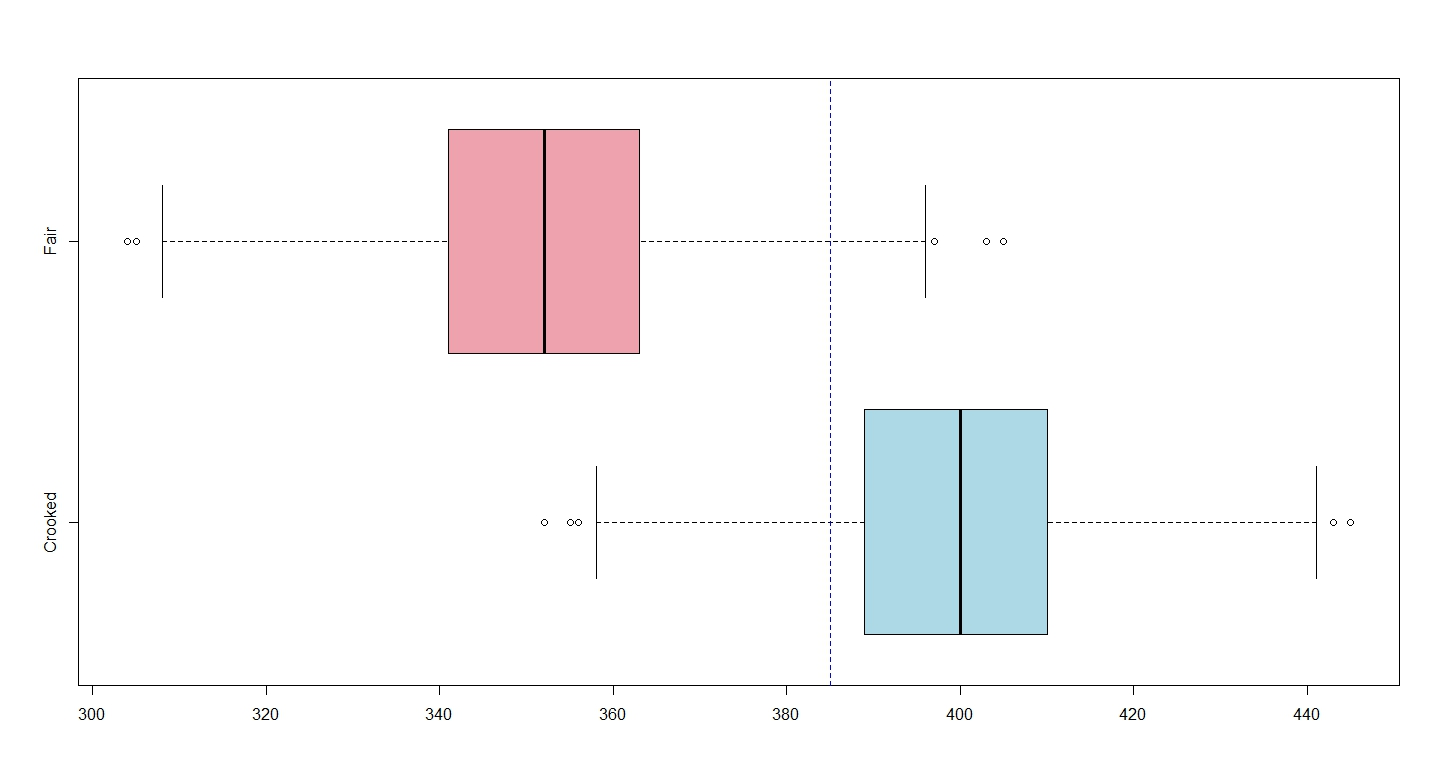
\includegraphics[width=0.7\linewidth]{./DiceBoxplot}
\caption{}
\label{fig:DiceBoxplot}
\end{figure}

\newpage
\begin{framed}
\begin{verbatim}
FairDice <- 1:6
CrookedDice<-c(1,2,3,4,4,5,5,6,6)

######################################################



Fair=numeric()
Crook=numeric()    # Initialize An Empty Vector
M=1000  # Number of Iterations

#FOR loop 
for (i in 1:M)
    {
     #Generate a New Value
     FairSum=sum(sample(FairDice,100,replace=TRUE))
     CrookSum=sum(sample(CrookedDice,100,replace=TRUE))
     
     #Add it to the record
     Fair = c(Fair, FairSum)
     Crook = c(Crook,CrookSum)

     }

######################################################


DiceSums = data.frame(
     Sums=c(Fair,Crook),
     DiceType=as.factor(c(rep("Fair",1000),
          rep("Crooked",1000) ))
     )


######################################################
boxplot(DiceSums$Sums~DiceSums$DiceType,
   horizontal=T,col=c("lightblue","lightpink2"))

abline(v=385,col="blue",lty=2)
\end{verbatim}
\end{framed}
%-----------------------------------------------------------------------------------------------------------------------------------%
\newpage
\section{The \texttt{prob} package}

The sample space of a coin toss experiment can be written out using the \texttt{tosscoin()} function on the \texttt{prob} package, specifying the number of tosses. The size of the sample space is $2^n$ for $n$ coin tosses, for binary outcome experiments. For 8 coin tosses, the sample space contains 256 possible outcomes.

\begin{verbatim}
> tosscoin(1)
  toss1
1     H
2     T
> tosscoin(2)
  toss1 toss2
1     H     H
2     T     H
3     H     T
4     T     T
\end{verbatim}
There is a similar command for dice roll : \texttt{rolldie()}. Again, specify the number of rolls. For $n$ dice rolls, there are $6^n$ outcomes in the sample space. (It gets large very quickly).

\begin{verbatim}
> rolldie(1)
  X1
1  1
2  2
3  3
4  4
5  5
6  6
\end{verbatim}

The \texttt{cards()} command describes each card from a deck of cards. The \texttt{roulette()} commands describes each possible spin from a roulette wheel.
\newpage
\subsection{The \texttt{prob} package : computing probabilities}
We can evaluate the probability associated with each sample point using the \texttt{makespace} argument.
\begin{verbatim}
> rolldie(1,makespace=TRUE)
  X1     probs
1  1 0.1666667
2  2 0.1666667
3  3 0.1666667
4  4 0.1666667
5  5 0.1666667
6  6 0.1666667
>
> tosscoin(3,makespace=TRUE)
  toss1 toss2 toss3 probs
1     H     H     H 0.125
2     T     H     H 0.125
3     H     T     H 0.125
4     T     T     H 0.125
5     H     H     T 0.125
6     T     H     T 0.125
7     H     T     T 0.125
8     T     T     T 0.125
\end{verbatim}
We can use this to compute the probability of certain events. Suppose we wish to compute the probability of a sum of 28 or more from five dice rolls. Importantly, each column of the output has a name. X1, X2 etc. Lets subset the sample space such that the sum of the 5 X variables is greater than or equal to 28. 
\begin{framed}
\begin{verbatim}
subset(rolldie(5,makespace=TRUE), X1 + X2 + X3 + X4 + X5 >= 28)
X = subset(rolldie(5,makespace=TRUE), X1 + X2 + X3 + X4 + X5 >= 28)
names(X)
X$prob
sum(X$prob)
\end{verbatim}
\end{framed}
\newpage
\begin{verbatim}
> X = subset(rolldie(5,makespace=TRUE), X1 + X2 + X3 + X4 + X5 >= 28)
> names(X)
[1] "X1"    "X2"    "X3"    "X4"    "X5"    "probs"
>
> X$prob
 [1] 0.0001286008 0.0001286008 0.0001286008 0.0001286008
 [5] 0.0001286008 0.0001286008 0.0001286008 0.0001286008
 [9] 0.0001286008 0.0001286008 0.0001286008 0.0001286008
[13] 0.0001286008 0.0001286008 0.0001286008 0.0001286008
[17] 0.0001286008 0.0001286008 0.0001286008 0.0001286008
[21] 0.0001286008
>
>
 sum(X$prob)
[1] 0.002700617
\end{verbatim}

%-----------------------------------------------------------------------------------------------------------------------------------%
\newpage
\subsection{The \texttt{prob} package ; Cards example}
Compute the probability of a King or Queen.
\begin{framed}
\begin{verbatim}
S <- cards(,makespace=TRUE)
subset(S, rank %in% c("Q","K"))
\end{verbatim}
\end{framed}

\begin{verbatim}
> subset(S, rank %in% c("Q","K"))
   rank    suit      probs
11    Q    Club 0.01923077
12    K    Club 0.01923077
24    Q Diamond 0.01923077
25    K Diamond 0.01923077
37    Q   Heart 0.01923077
38    K   Heart 0.01923077
50    Q   Spade 0.01923077
51    K   Spade 0.01923077
\end{verbatim}

\begin{verbatim}
> X = subset(S, rank %in% c("Q","K"))
> sum(X$probs)
[1] 0.1538462
\end{verbatim}
\newpage
%-----------------------------------------------------------------------------------------------------------------------------------%

\newpage
\section{Gambler's Fallacy}

\begin{figure}[h!]
\centering
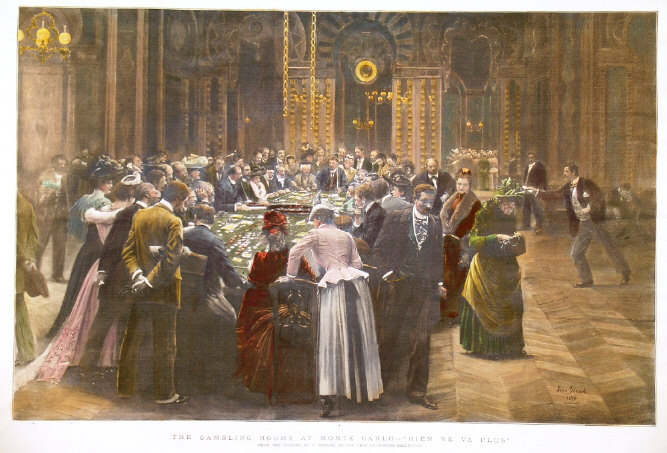
\includegraphics[width=0.7\linewidth]{./Gamblers}
\caption{}
\label{fig:Gamblers}
\end{figure}

The \textbf{\textit{Gambler's fallacy}}, also known as the \textbf{\textit{Monte Carlo fallacy}} (because its most famous example happened in a Monte Carlo Casino in 1913),and also referred to as the fallacy of the maturity of chances, is the belief that if deviations from expected behaviour are observed in repeated independent trials of some random process, future deviations in the opposite direction are then more likely. \textit{(Wikipedia)}
\subsection{Monte Carlo Casino}\begin{figure}
\centering
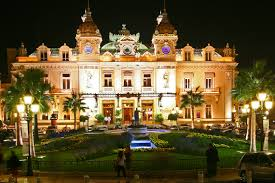
\includegraphics[width=0.7\linewidth]{./MonteCarlo}
\caption{}
\label{Monte Carlo}
\end{figure}

The most famous example of the gambler’s fallacy occurred in a game of roulette at the Monte Carlo Casino on August 18, 1913, when the ball fell in black 26 times in a row. This was an extremely uncommon occurrence, although no more nor less common than any of the other 67,108,863 sequences of 26 red or black. Gamblers lost millions of francs betting against black, reasoning incorrectly that the streak was causing an "imbalance" in the randomness of the wheel, and that it had to be followed by a long streak of red. \textit{(Wikipedia)}
\newpage
\subsection{Implementation with \texttt{R}}
Firstly let simulate the outcomes of a Roulette Wheel.
\begin{itemize}
\item  For the sake of simplicity, we will disregard "Green" and let ``Black" be signified by an outcome of 1 and ``Red" signified by an outcome of 2.
\item 
For this we will use the \texttt{runif()} command, as well as the \texttt{ceiling()} command, which rounds a value up to the next highest integer.
\end{itemize}
\begin{framed}
%------------------------------------------------------ %
\begin{verbatim}
runif(5)
2*runif(5)
ceiling(2*runif(5)) #Ones and Twos
\end{verbatim}
\end{framed}
\begin{verbatim}
> runif(5)
[1] 0.02646220 0.90602044 0.45596144 0.25390162 0.06416899
> 
> 
> 2*runif(5)
[1] 1.4458583 0.7452968 0.7861305 0.4930401 1.9711546
> ceiling(2*runif(5))
[1] 2 2 2 1 1
\end{verbatim}
In this last code segment, we get ``Red" three times in a row, and  then two "Blacks". Try it for a larger number of trials.(e.g. 100)
\begin{framed}
\begin{verbatim}
ceiling(2*runif(1000))
\end{verbatim}
\end{framed}

\begin{itemize}
\item What is of interest is the number of repeated colours. What we could do is to construct a \texttt{For} loop so as to monitor how often a colour repeats.

\item Each time a new colour comes up, the sequence counter gets set to 1. If the next spin results in the same colour, the sequence number is set to 2, if it happens again, the next sequence number is 3, and so on.

\item Firstly let set up a basic \texttt{FOR} loop to generate the colours. Ths code is more elaborate than the approach we used already, but it is easy to use this for studying repetitions.
\end{itemize}

\begin{framed}
\begin{verbatim}
M=100

#First Spin
Colour=ceiling(2*runif(1))

for(i in 2:M)
  {
  # Next Colour
  NextCol =  ceiling(2*runif(1))
  Colour = c(Colour,NextCol)
  }
\end{verbatim}
\end{framed}
\begin{verbatim}
> Colour
  [1] 2 2 2 2 1 1 2 2 1 1 2 1 1 1 2 1 2 2 1 2 1 2 2 1 2 1 2 1 2 1
 [31] 1 1 2 2 2 1 2 2 1 2 2 1 2 2 2 1 1 1 1 2 2 1 2 2 2 2 1 1 2 2
 [61] 1 2 1 2 1 2 2 2 1 1 2 2 1 2 1 1 2 1 2 1 2 2 2 1 1 2 2 1 1 2
 [91] 1 1 2 2 1 2 1 1 2 2
\end{verbatim}

\newpage
We are going to do something similar here, but record the sequence lengths.
\begin{framed}
\begin{verbatim}
M=100

#First Spin
Colour=ceiling(2*runif(1))


# Start a vector with a single value of 1.
SeqNo=c(1)  

for(i in 2:M)
  {
  # Next Colour
  NextCol =  ceiling(2*runif(1))
  Colour = c(Colour,NextCol)
  

  #If the current colour is the same as the last, then the current 
  #value in the sequence number vector  is 1 more than the last.
  #
  #Otherwise the current sequence number is reset to 1.
  if (Colour[i] == Colour[i-1])
    {
    SeqNo[i] = SeqNo[i-1]+1
    }else SeqNo[i]=1
  }
\end{verbatim}
\end{framed}
\newpage
\begin{verbatim}
> max(SeqNo)
[1] 5
>
> cbind(Colour,SeqNo)
       Colour SeqNo
  [1,]      2     1
  [2,]      2     2
  [3,]      2     3
  [4,]      1     1
  [5,]      2     1
  [6,]      2     2
  [7,]      1     1
  [8,]      1     2
  [9,]      2     1
 [10,]      1     1
\end{verbatim}
To reduce data that needs to be collected, we will look at a \textit{Sequence Maximum}. 
\begin{itemize}
\item If there is a change of colour, the last sequenc number is added to a special vector:  \texttt{SeqMax}. 
\item For the sake of brevity, Any values lower than 3 in \texttt{SeqMax }will be discarded afterwards.
\end{itemize}
%---------------------------------%
\newpage
\begin{framed}
\begin{verbatim}
M=100

#First Spin
Colour=ceiling(2*runif(1))
SeqNo=c(1)

SeqMax=numeric()

for(i in 2:M)
  {
  # Next Colour
  NextCol =  ceiling(2*runif(1))
  Colour = c(Colour,NextCol)


  if (Colour[i] == Colour[i-1])
    {
    SeqNo[i] = SeqNo[i-1]+1
    }else{SeqNo[i]=1;SeqMax=c(SeqMax,SeqNo[i-1])}
}	
SeqMax = SeqMax[SeqMax>3]
\end{verbatim}
\end{framed}
Increase the number of iterations to a large number, say 100,000. Then see what turns up in the \texttt{SeqMax} vector. Use the \texttt{table()} command to determine the distribution.
\begin{verbatim}
> table(SeqMax[SeqMax>10])

11 12 13 14 15 18 
21  6  2  3  1  1 
\end{verbatim}
%-----------------------------------------------------------------------------------------------------------------------------------%
\newpage
\section{Gambler's Ruin}
Consider a gambler who starts with an initial fortune of $A$ dollars and then on each successive gamble
either wins  or loses independent of the past with probabilities $p$ and $q = 1- p$ respectively.
This gamblers places bets with the Banker, who has an initial fortune of $B$ dollars. 

(For the sake of simplicity, we will look at the game from the perspective of the gambler only. The Banker is, by convention, the richer of the two (i.e. A<B) , and has a better chance of winning.)

\begin{itemize}
\item Probability of successful gamble for gambler : $p$
\item Probability of unsuccessful gamble for gambler : $q$ (where $q = 1 - p$ )
\item Ratio of success probability to failure success: $s = p/q$
\item Conventionally the game is biased in favour of the Banker (i.e.$ q > p$ and $s < 1$)
\end{itemize}


\subsection{Simulating a Single Gamble}
To simulate one single bet, compute a single random number between 0 and 1. For this, we 
use the \texttt{runif()} command, which uses generates a \textbf{\textit{continuous uniform random variable}}. The upper and lower limits can be specified. In the absence of particular specifications, the defaults are 0 and 1.
\begin{framed}
\begin{verbatim}
runif(1)
\end{verbatim}
\end{framed}
Lets assume that the game is biased in favour of the Banker with $p = 0.45$ ,$q = 0.55$. If the
number is less than 0.45, the gamble wins. Otherwise the Banker wins.
\begin{verbatim}
> runif(1)
[1] 0.1251274
>#Gambler Wins
>
> runif(1)
[1] 0.754075
>#Gambler loses
>
> runif(1)
[1] 0.2132148
>#Gambler Wins
>
> runif(1)
[1] 0.8306269
>#Gambler Loses
\end{verbatim}
\newpage
%---------------------------------------------------%
\subsection{Repeated Gambles}
Let A be the Gambler's Kitty at the start of the gambling. Let B be the Banker's Wealth at the outset. (Therefore the total jackpot is A+ B )
The probability of gambler winning a gamble is $p$.

\begin{itemize}
\item Let $Rn$ denote the Gamblers total fortune after the $n-$th gamble. If the Gambler wins the first game, his wealth becomes $Rn$ = $A + 1$. 
\item If he loses the first gamble, his wealth becomes $Rn$ = $A - 1$. The entire sum of money at stake is the Jackpot i.e. $A + B$. 
\item The game ends when the Gambler wins the Jackpot ($Rn = A + B$) or loses everything ($Rn = 0$).
\item The vector \texttt{Rec} records the gambler's worth on an ongoing basis, with the first element being the value of $A$. As the gambling progresses, the new value gets added to the vector.
\end{itemize}

Lets see how this plays out over a night of gambling. Let's start the gambler with 20 dollars, and the banker with 100. Unknown to the gambler is the fact that he or she has only a 47\% chance of winning a single bet at each round.
\begin{framed}
\textbf{Basic Structure}
\begin{verbatim}
#initial values
A=20;B=100;p=0.47

#record the progress of the gambler - who starts with A wealth
Rec=c(A)

#generate a outcome for each gamble.
probval = runif(1)

if (probval < p)
{
A = A+1; B =B-1
}else{A=A-1;B=B+1}

#Save the values from each bet
Rec=c(Rec,A)
\end{verbatim}
\end{framed}
%-----------------------------------------------------------------------%
\newpage
\subsection{Using a \texttt{while} loop}
So far we have managed to code for a single bet. Lets simulate the gambling in its entirety.
For this, we will use a \texttt{while} loop. A \texttt{while} loop will repeat a set of commands as long as a particular logical condition is met. (Here, that logical condition is that the gambler has money to gamble with i.e. $A >0$). Once he loses everything, the \texttt{while} loop (and the gambling) terminates.
\begin{framed}
\begin{verbatim}
A=20;B=100;p=0.47
Rec=c(A)

while(A>0)
{
    ProbVal=runif(1)
    if(ProbVal <= p)
      {
      A = A+1; B =B-1
      }else{A=A-1;B=B+1}
    Rec=c(Rec,A)

}
\end{verbatim}
\end{framed}
We will also include a \texttt{break} statement to stop the loop in the unlikely event that the Gambler wins the jackpot.
\begin{framed}
\begin{verbatim}
A=20;B=100;p=0.47
Rec=c(A)
Total=A+B  #total jackpot

while(A>0)
   { 
   ProbVal=runif(1)
   if(ProbVal <= p)
   {
   A = A+1; B =B-1
   }else{A=A-1;B=B+1}
   Rec=c(Rec,A)
   if(A==Total){break}
   }
\end{verbatim}
\end{framed}
\newpage
\subsection{The Gambler's Performance}
In all likelihood, the Gambler lost everything. But how long did he last in the game? how many gambles was he able to play? Also What was his highest level of wealth?
We can look at the \textbf{\textit{Rec}} vector to answer these questions.
\begin{framed}
\begin{verbatim}
length(Rec)
max(Rec)
\end{verbatim}
\end{framed}
We are going to write a function, called \texttt{GambRuinFunc()} to produce a duration value, for given values of $A$, $B$ and $p$. 
\begin{framed}
\begin{verbatim}
GambRuinFunc=function(A=20,B=100,p=0.47)
{
Rec=c(A)
Total=A+B  #total jackpot

while(A>0)
   { 
   ProbVal=runif(1)
   if(ProbVal <= p)
   {
   A = A+1; B =B-1
   }else{A=A-1;B=B+1}
   Rec=c(Rec,A)
   if(A==Total){break}
   }
return(length(Rec))
}
\end{verbatim}
\end{framed}



We can construct a plot to depict the gambler's ongoing fortunes in the game.
\begin{framed}
\begin{verbatim}
# Line plot, colour red
plot(Rec,type="l",col="red")

#Axes
abline(h=0)
abline(v=0)

#Also the gamblers initial value and the total value of the game(optional)
abline(h=A,col="red")
abline(h=Total,col="green")
\end{verbatim}
\end{framed}
\newpage
\subsection{Simulation Study}
Suppose we are interested in the probability distribution of durations. What is the probability of lasting more than 100 rounds? less than 200 etc? We can use a function called \texttt{GambRuinFunc()} to compute the durations from an number of nights of gambling (next page) . The function can easily be adjusted to consider the maximum value of the gambler's worth
We can specify values for A , B and p different to that of the defaults. Here, they are picked so as to be quick to execute.
\begin{framed}
\begin{verbatim}
Durations= numeric()
M=1000
for(i in 1:M)
   {
   NextDuration = GambRuinFunc(A=10,B=30,p=0.40)
   Durations=c(Durations,NextDuration)
   } 
\end{verbatim}
\end{framed}

We can study the Durations vector  using simple statistical functions.
\begin{framed}
\begin{verbatim}
hist(Durations)
mean(Durations)
median(Durations)
IQR(Durations)
quantile(Durations,1:20/20)
\end{verbatim}
\end{framed}


\newpage
\begin{framed}
\begin{verbatim}
GambRuinFunc=function(A=20,B=100,p=0.47)
{
Rec=c(A)
Total=A+B  #total jackpot

while(A>0)
   { 
   ProbVal=runif(1)
   if(ProbVal <= p)
   {
   A = A+1; B =B-1
   }else{A=A-1;B=B+1}
   Rec=c(Rec,A)
   if(A==Total){break}
   }
Duration=length(Rec)
return(Duration)
}
\end{verbatim}
\end{framed}
We are going to keep track of the time it takes to carry out this simulation.
\begin{framed}
\begin{verbatim}
Time1=Sys.time()
DurDist=numeric()
M=150000
for(i in 1:M){ 

 DurDist=c(DurDist,GambRuinFunc())
 }

Time2=Sys.time()
#

hist(DurDist,main="Durations Distribution",breaks=100)
quantiles(DurDist)
\end{verbatim}
\end{framed}
\newpage

\begin{framed}
\begin{verbatim}
hist(Durations)
mean(Durations)
median(Durations)
IQR(Durations)
quantile(Durations,1:20/20)
\end{verbatim}
\end{framed}


\newpage
\begin{framed}

\begin{verbatim}
GambRuinFunc=function(A=20,B=100,p=0.47)
{
Rec=c(A)
Total=A+B  #total jackpot

while(A>0)
   { 
   ProbVal=runif(1)
   if(ProbVal <= p)
   {
   A = A+1; B =B-1
   }else{A=A-1;B=B+1}
   Rec=c(Rec,A)
   if(A==Total){break}
   }
Duration=length(Rec)
return(Duration)
}
\end{verbatim}
\end{framed}
\begin{verbatim}
> quantile(DurDist)
  0%  25%  50%  75% 100% 
  23  139  239  419 4167 
> 
> quantile(DurDist,1:10/10)
 10%  20%  30%  40%  50%  60%  70%  80%  90% 100% 
  91  123  157  195  239  295  369  481  691 4167 
\end{verbatim}
\newpage
\begin{figure}[h!]
\centering
\includegraphics[width=0.85\linewidth]{../DurDist}
\caption{}
\end{figure}
\begin{figure}[h!]
\centering
\includegraphics[width=0.85\linewidth]{../DurDist2}
\caption{}
\label{Same - Without Upper Tail}
\end{figure}
%-----------------------------------------------------------------------------------------------------------------------------------%
\end{document}
